\documentclass[11pt]{article}
\usepackage[ngerman]{babel}
\usepackage[left=3cm,right=3cm,top=3cm,bottom=3cm]{geometry}
\usepackage[utf8]{inputenc}
\usepackage[T1]{fontenc}
\usepackage{amsmath}
\usepackage{amssymb}
\usepackage{hyperref}
\usepackage{graphicx}
\usepackage{xcolor,listings}


% Used to reference java classes
\newcommand{\class}[1]{{\color{green!50!black}\small\texttt{#1}}}
% Used to reference files or folders in the git/project directory
\newcommand{\source}[1]{{\color{blue!80!white}\texttt{\lstinline|#1|}}}

\begin{document}
	\begin{titlepage}
		\begin{center}
			\title{Project Report: BamBirds 2019\\
				{\small Creating  an Intelligent Game Playing Agent for Angry Birds}}
			
\includegraphics[width=3cm,height=3cm]{img/logo.png}
			\author{Samet\\Akcabay\and
			Patrick\\Haller}
		\end{center}
	\end{titlepage}
\maketitle
\newpage
\tableofcontents
\newpage
xi
% Patrick 
\section{Aufgabenstellung des Smart Environment Projekts}
AngryBirds, ein in 2009 von Rovio Entertainment entwickeltes Casual-Puzzle-Videospiel, ist ideal als Maßstab für künstliche Intelligenz geeignet. Der Weg zum Erfolg setzt voraus, dass ein Verständnis der physikalischen Zusammenhänge auf das Spiel übertragen werden können und strategische Entscheidungen getroffen werden müssen. Ziel des Projekts war es, die Schwächen des BamBirds-Agenten zu verbessern und um Funktionen zu erweitern, um mit diesem an der Angry Birds AI Competition teilnehmen zu können und diesen zu gewinnen.\\Parallel zu diesem Wettkampf, lief die sogenannte AIBirds COG 2019 Level Generation Competition, in welchem das Ziel daraus bestand, mit einem selbsterstellten Programm der Wahl, automatisiert Level zu generieren, welche viel Spaß und Herausforderung anbieten sollen. Dieser Aufgabe haben wir uns gewidmet.

% Patrick (Motivation, Bilder)
\section{Machine Learning als möglicher Levelgenerator}
\subsection{Hintergrund [wie ist Patrick drauf gekommen?]}
Im Gegensatz zu dem gegebenen Levelgenerator, wollten wir einen Ansatz wählen, der nicht auf prozedualer Generieriung beruht, sondern mit Machine Learning Techniken arbeitet. 

Der Generator soll anhand von bestehenden Leveln lernen und daraus neue generieren.


\subsection{Generative Adversial Networks (GAN)}
Generative Adverserial Networks, kurz GAN (zu deutsch "erzeugende generische Netzwerke"), stellen in der Informatik eine Gruppe von Algorithmen zu unüberwachtem Lernen dar. Sie bestehen aus zwei Neuronalen Netzwerken, eines erstellt Kandidaten (\textbf{Generator}), das zweite bewertet diese (\textbf{Diskriminator}).\\Der Generator lernt, Ergebnisse nach einer bestimmten Verteilung zu erzeugen. Der Diskriminator hingegen lernt, die Ergebnisse des Generators gegen die echte, vorgegeben Verteilung zu evaluieren (hier: konkret spielbare Level). Findet der Diskriminator keine Unterschiede mehr im direkten Vergleich der vorgegebenen Verteilung, so wird das Ziel erreicht.\\Neuronale Netzwerke kommen häufig zur Visualisierung verschiedener Gegenstände, zur Erstellung von 2D- bzw. 3D-Modellen oder zur Bildbearbeitung (astronomischer Bilder) zum Einsatz.\\Aus diesem Grund entschieden wir uns für GAN als geeigneten Kandidaten eines Level-Generators.
\subsection{...}

% Samet
\section{Allgemeine Vorgehensweise}
Im Folgenden wird die allgemeine Vorgehensweise beschrieben. Zur besseren Strukturierung, Dokumentierung und klaren Aufgabenverteilung, haben wir uns ein eigenes GitHub-Repository \footnote{https://github.com/HallerPatrick/AI-Birds-LeveGANerator} aufgesetzt, in welchem ebenfalls die Arbeitszeiten an den bestimmten Issues festgehalten wurden. Die wichtigsten Aufgaben werden in den nachfolgenden Unterkapiteln näher erläutert. [Graphen, allgemeine Struktur]
\begin{figure}
    \centering
    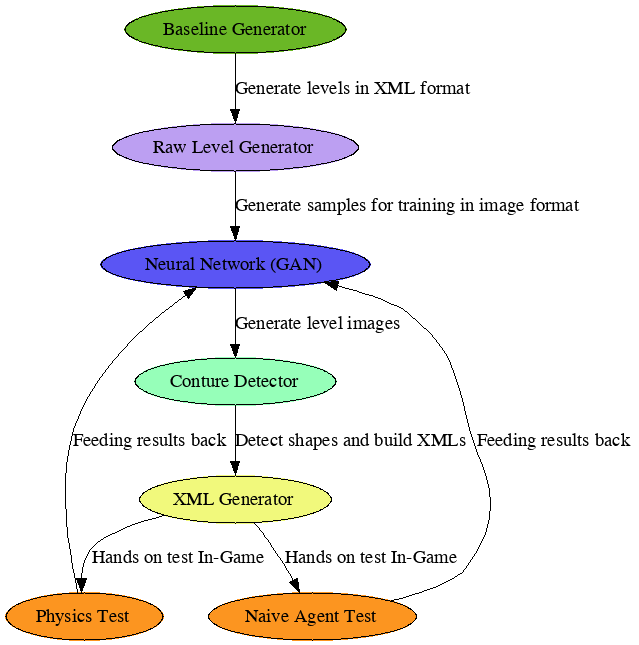
\includegraphics[height=12cm, width=10cm]{img/project_structure.png}
\end{figure}
\subsection{Erkennen der  Konturen von Zentroiden}
Um generell mit den generierten Bildern arbeiten zu können war es wichtig, diese erst durch die Erzeugung und Verstärkung der Konturen besser auf den Konturenerkenner abzustimmen. Nachfolgend möchten wir die Klasse \textit{conture\_detector.py} näher erläutern. \\
Zur allgemeinen Verarbeitung der Bilder bedarf es eines Imports der cv2-Klasse, welches zuvor installiert werden muss (unter OS X und Python3: \textit{"pip3 install opencv-python"}). In der Klasse wird nun das Bild ausgelesen und alle x- sowie y-Koordinaten in eine Liste \textit{*points} geschrieben. Das eingelesene Bild im HSV-Farbraum ("\textbf{h}ue": Farbwert, "\textbf{s}aturation": Farbsättigung, "\textbf{v}alue": Hell-/Dunkelwert)\footnote{https://de.wikipedia.org/wiki/HSV-Farbraum} wird in Graustufen umgewandelt, um Konturen innerhalb des Bildes zu ermöglichen (dieser Schritt kann allerdings auch übersprungen werden, da die Objekte verschiedene Farben aufweisen). \\ Zur Ermittlung der Zentroiden wird nun die Formel \[centrX = \sum XCoord / Length\] wobei folgende Zuweisungen gelten:
\begin{itemize}
	\item \(centrX\) entspricht den zu ermittelnden Zentroiden der X-Koordinaten (gilt analog für Y-Koordinaten mit \(centrY\))
	\item  \(\sum XCoord\) entspricht der Summe aller X-Koordinaten (gilt analog für Y-Koordinaten mit \(\sum YCoord\))
	\item  \(Length\) entspricht der Länge aller Punkte
\end{itemize}
\begin{figure}
	\centering
	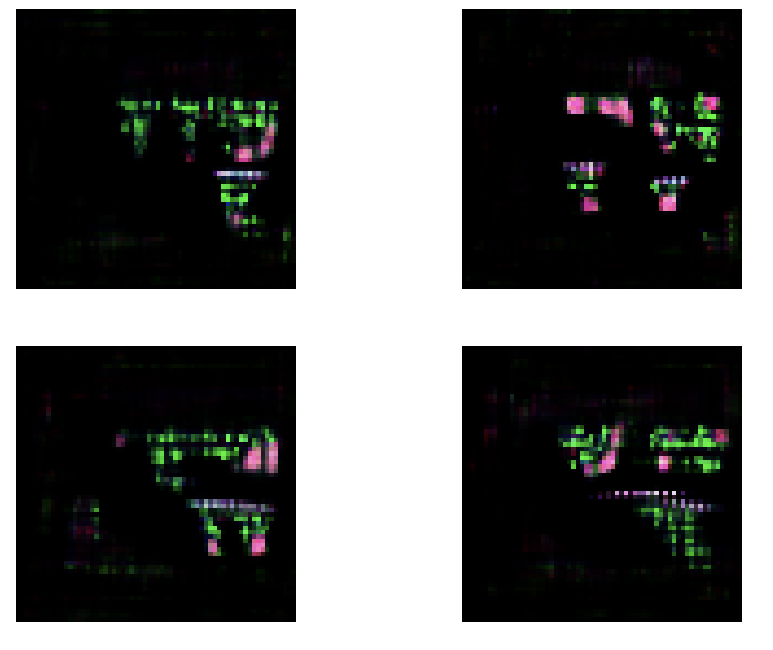
\includegraphics[height=10cm, width=10cm]{img/blurry_attempts.png}
	\caption{Verschwommene Konturen führen zu Problemen bei der Erkennung}
\end{figure}
\subsection{Automatisierung der Abläufe mithilfe von Powershell unter Windows}
Um zu vermeiden, dass alle Komponenten einzeln und umständlich gestartet werden müssen, haben wir es uns außerdem zur Aufgabe gemacht, ein Automatisierungsskript aufzusetzen, welcher diesen Schritt für uns übernimmt. Als Skriptsprache erschien uns PowerShell am sinnvollsten, da dieses ein fester Bestandteil von Windows 10 (dem gängigsten Betriebssystem) ist und aufgrund dessen keine extra Tools installiert und erläutert werden müssen. \\Das Skript startet zunächst ScienceBirds und skaliert diesen mithilfe von Window-Resizer (Tool zur nutzerbasierten Steuerung der Standardgröße eines Fensters, hier: ScienceBirds) auf einen bestimmten Wert, da der Agent sonst mit der Größe des ScienceBirds-Fensters nicht einverstanden ist. Im Anschluss wird der Agent und der Server automatisch in der Eingabeaufforderung gestartet. Wir konnten beobachten, dass durch den Startklick des Skripts alle benötigten Fenster ordnungsgemäß gestartet wurden und der Agent das Spiel wie erwartet, selbstständig gespielt hat.\\ In den folgenden Stichpunkten werden die einzelnen Fenster der Automatisierung näher erläutert (vgl. Abb.1).
\begin{itemize}
	\item[1)] Shell des Automators \\
	Aus diesem Fenster wird der Automator gestartet. Dazu wird zunächst überprüft, ob alle Umgebungsvariablen vorhanden und passend eingestellt sind, um volle Funktionalität gewährleisten zu können. Findet der Automator alle benötigten Tools, so wird der Nutzer gefragt, ob er diesen starten, den Vorgang abbrechen oder Umgebungsvariablen einstellen möchte.
	\item[2)] ScienceBirds-Fenster \\
	In diesem Fenster läuft das eigentliche Spiel. Da die Größe dieses Fensters für unseren Agenten nicht gepasst hat, musste ein Window-Resizer eingeschaltet werden, um ScienceBirds auf die benötigte Fenstergröße zu skalieren.
	\item[3)] AutoSizer-Fenster \\
	Hier befindet sich unser Window-Resizer. Dabei haben wir uns für den AutoSizer als Tool entschieden, da dieser wenig Speicherplatz einnimmt, kostenlos und ohne Bloatware zu installieren ist. Damit die Größe eines spezifischen Fensters auf einen immer gleichbleibenden Wert angepasst werden muss, haben wir im AutoSizer selbst einen Hotkey festgelegt, welcher beim Betätigen einer bestimmten Tastenkombination (hier: "\%9") die Größe von einem Fenster mit dem Namen "ScienceBirds" auf die benötigte Auflösung ändert. Diese Methode ist stark auf unser persönliches System abgestimmt, kann aber durch wenige Änderungen im Skriptcode auf die eigenen Parameter angepasst werden.
	\item[4)] Agent-Fenster \\ 
	Hieraus wird der Agent gestartet. Dazu wird zuerst der Agent gestartet und im Anschluss darauf der Server. Hier lässt sich beobachten, dass sich der Status von "Waiting" auf "Pending" ändert. Startet man nun den Agenten mit dem Klick auf "Start", so wechselt der Agent in den Status "Running".
	\item[5)] Server-Fenster
	Der Server muss gestartet werden um gewährleisten zu können, dass der Agent ordnungsgemäß läuft. Hier kann man die verschiedenen Aktionen beobachten, welche gerade stattgefunden haben (hier: "Go to Level Selection Page").
\end{itemize}
\begin{figure}
	\centering
	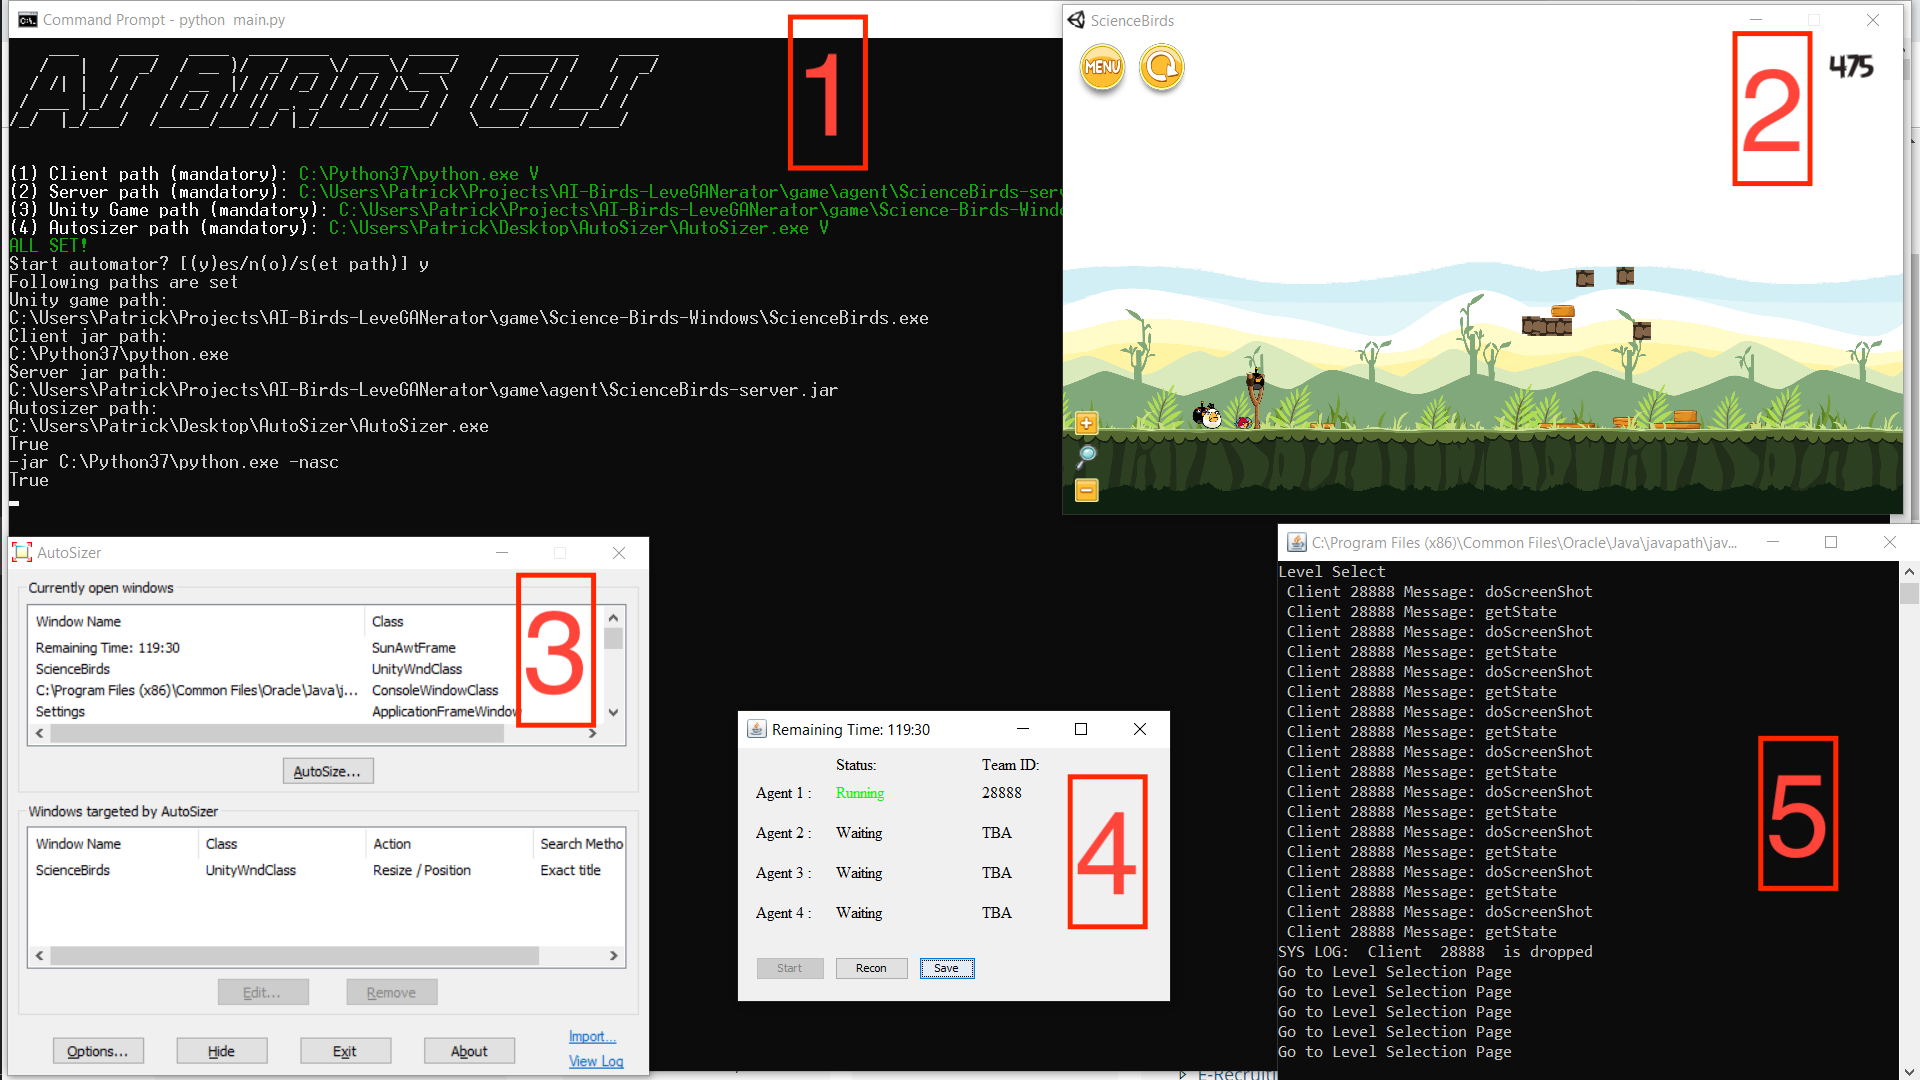
\includegraphics[height=9cm, width=16cm, clip]{img/automator_screen.png}
	\caption{Vorläufige GUI der Automatisierung}
\end{figure}
\subsection{Konvertierung von Pillow-Koordinaten in ein kartesisches XML-Koordinatensystem}
[Patrick]
\subsection{Verdeutlichen der Konturen der erzeugten RAW-Bilder zur besseren Erkennung vor Training}
Der Konturen-Erkenner hatte in unserem Durchlauf Probleme, die Umrisse der erzeugten Zentroide zu erkennen. Aufgrund dessen mussten wir die Konturen, welche erzeugt werden, vor dem Beginn des Trainings verstärken, damit diese eindeutig von unserem Erkenner gefasst werden können. 
\subsection{Aufsetzen eines Re-Evaluierungssystems}
[Patrick]

% Samet

\section{Ergebnisse}
Wir haben unsere Generative Adversial Networks nun zur Generierung von Plattformen, Schweinen, TNTs und Blöcke eingesetzt. Dabei stellen wir für die verschiedenen Gegenstände fest, dass unterschiedliche Ergebnisse erzielt wurden. Im ersten Fall widmen wir uns den Plattformen. Bei diesen fällt auf, dass aus dem Ursprungsbild Konturen herausstechen und eine Form annehmen. In unserem Beispiel haben wir knapp sechs Tausend, sich immer weiter verbessernde Bilder generieren lassen. Auffällig dabei ist jedoch, dass die Konturen und Formen, die Plattformen darstellen sollen, immer flächenartiger werden und somit eine geeignete Grundlage darstellen sollten, diese allerdings in ihrer Struktur sinnfrei und zum Teil identisch mit einem vollständig flachen Level ist. Es sind weder Plattformen in der Höhe bzw. außergewöhnliche Formen aufzufinden, welche den Spielspaß verbessern könnten. \\ Anders sieht es hier bei den punktförmigen Gegenständen, wie den Schweinen und TNTs, aus. Diese können mithilfe des GAN bisher gut innerhalb des Levels verstreut werden. Es kommt weiterhin vor, dass Schweine sehr nah beieinander stehen und deshalb in den GAN als eine Linie generiert werden (si. Verdeutlichen der Konturen der erzeugten RAW-Bilder zur besseren Erkennung von Training). Leider besteht auch hier das Problem, dass Faktoren wie Spaß und Herausforderung (bisher) nicht eingebracht werden konnten, weswegen die Verteilung der einzelnen Objekte derzeit willkürlich ausfällt. Dieses Problem zieht sich auch durch die anderen Gegenstände. \\ \\Ein weiteres Problem stellt die Verteilung der punktförmigen Gegenstände dar. Am Beispiel der Schweine fällt diese auf den Blick zwar sinnvoll aus, da diese passend über das Level verstreut oder nachvollziehbar angeordnet sind. Nur häufig finden sich keine Blöcke unter den Gegenständen, sodass diese beim Start des Levels durch das Fallen entweder zwingend ihren Standort verändern oder sogar ohne Einwirkung des Spielers sofort sterben. Dies ist jedoch fatal für das Spielprinzip, da die Schweine nur durch die Aktionen des Spielers zu eliminieren sein sollten.
\section{Fazit}
Aus unseren Ergebnissen wird deutlich, dass GAN weniger zum Generieren von Level geeignet ist, da die erzeugten Level nicht sinnvoll sind. Das heißt, dass häufig obsolete Plattformen vorzufinden sind, welche in ihrem Aufbau und ihrer Struktur kein spielbares Level darstellen. Zudem erfolgt die Platzierung der Schweine und Hindernisse ohne jeglichen Wert auf Faktoren wie Spaß und Herausforderung zu legen, weswegen die generierten Level wenig für den Spieler bieten zu haben. Aufgrund dessen finden GANs ihren Einsatz oft nur bei der Erstellung photorealistischen Bildern zur Visualisierung verschiedener Gegenstände, bei der Modellierung von Bewegungsmustern in Videos, bei der Erstellung von 3D-Modellen von Objekten aus 2D-Bildern und bei der  Bildbearbeitung von astronomischen Bildern. Da unsere Methode der Neuronalen Netze keine brauchbaren Ergebnisse geliefert hat, wurde dieser beim Levelgenerator-Wettkampf nicht eingereicht. 
\section{Ausblick}
Für zukünftige Teams, die sich mit dem Projekt "AI Birds" des Lehrstuhls für Smart Environments befassen wollen, möchten wir als Abschluss Verbesserungsvorschläge des aktuellen Stands erläutern. Für die genannten Punkte bietet es sich an, den bereits vorhandenen Fortschritt zu verwenden und weiter auszubauen. Natürlich ist es aber auch möglich, komplett eigene Ansätze anzuwenden bzw. den vorhandenen Stand neu zu entwerfen. \\ Die Automatisierung der Abläufe funktioniert bereits einwandfrei und gemäß der Erwartungen. Trotzdem wäre es sinnvoll. eine GUI (z.B. mit JavaFX) zu entwerfen, um diesen Prozess überhaupt optisch darzustellen und dem Nutzer vor allem Übersicht über das Geschehen zu gewähren. Visuelles Feedback, was genau gerade passiert, wie weit der Automator vorangeschritten ist oder ob Fehler aufgetreten sind (mit genauem Fehlercode) sind sinnvolle Ergänzungen.
[Verbesserungsvorschläge][Wie kann man GAN passend für Level-Generierung gestalten?] [RNN als mögliche Alternative?]
\subsection{GAN im Vergleich zu Alternativen}
Im direkten Vergleich von GAN mit den Alternativen empfiehlt es sich, die Meinungen und Erfahrungen von Experten heranzuziehen, die diese auch in der Praxis umgesetzt und angewendet haben, um so am effektivsten darüber urteilen zu können, wie GAN in Abhängigkeit seiner Alternativen abschneidet. Im Folgenden möchten wir uns auf Alexandr Honchar beziehen, welcher selber Unternehmer und Praktiker mit künstlicher Intelligenz ist und selbst schon mit GAN und diversen Alternativen dazu gearbeitet hat. Honchar stellt in seinem Kommentar "GANs beyond generation: 7 alternative use cases", welches 2018 auf der Webseite Medium erschienen ist, sieben Alternativen zu GAN vor und bewertet diese nach eigener Einschätzung.\\ Im Folgenden beschränken wir uns der Übersichtlichkeit halber auf die ersten drei Beispiele. \\Zunächst stellt Honchar die Anhebung der Daten vor, in welcher das Model im Model-View-Controller so trainiert wird, dass neue Beispieldaten von den bereits existierenden und zu verbessernden Daten generiert werden. Dies wird durch zwei Strategien erreicht: In der ersten wird das Model durch simulierte Daten trainiert und im Anschluss überprüft, welche Ergebnisse mit echten Beispieldaten erzielt werden. Die zweite Strategie auf der anderen Hand setzt auf echte Daten zum trainieren und wird dann mit den generierten Daten verglichen (Überschneidung mit GAN). \\ Als zweiten Punkt ... [...]


\end{document}
